\section{Assumptions}

This thesis posits the existence of high-level musical concepts invariant to specific attributes such as sound quality, tempo, key, orchestration, and signal noise that evolve and unfolds through time. This idea parallels the nature of the symbolic domain (sheet music), which maintains its essence despite being interpreted through diverse performances using various instruments and styles. While a single waveform might have a limited number of sheet music representations that adequately capture its musical components, a single piece can be interpreted in infinite ways through different instruments, voices, tempos, and interpretations. The distinct tonal quality of a waveform, heavily influenced by the specific timbre of the instrument or production technology, adds complexity to the transcription of its sonic properties into accurate sheet music notation.

Abstract high-level features can be discerned regardless of waveform or production style. This approach provides an objective, comprehensive insight into a composition's musical content and meaning, much like analyzing sheet music uncovers its intentional foundation.

For example, despite the differences in cultural contexts, stylistic elements, time signatures, key signatures, and sonic properties, we propose that figures \ref{fig:mahler} and \ref{fig:giant_steps} share a similarity. Both pieces carry the same musicological fingerprint so to say, derived from the propulsion of their melodic and harmonic contours through non-diatonic major thirds.

This concept finds grounding in the theories of Kurt Koffka, a founder of the Gestalt school of psychology, who proposed a holistic approach to understanding complex forms, contrary to the structuralist practice of reducing mental processes into essential elements \cite{Koffka2013PrinciplesPsychology}.

When applied to music, the principles of Gestalt psychology offer insights into how we perceive, organize, and interpret musical patterns. They suggest that our minds perceive auditory input much like visual input, seeking patterns and structures. This understanding significantly contributes to the comprehension of cognitive processes in musical perception and organization, influencing music theory, cognition, and therapy \cite{Lerdahl1985AMusic}.

\begin{figure}[ht]
    \centering
    \scalebox{0.9}{
    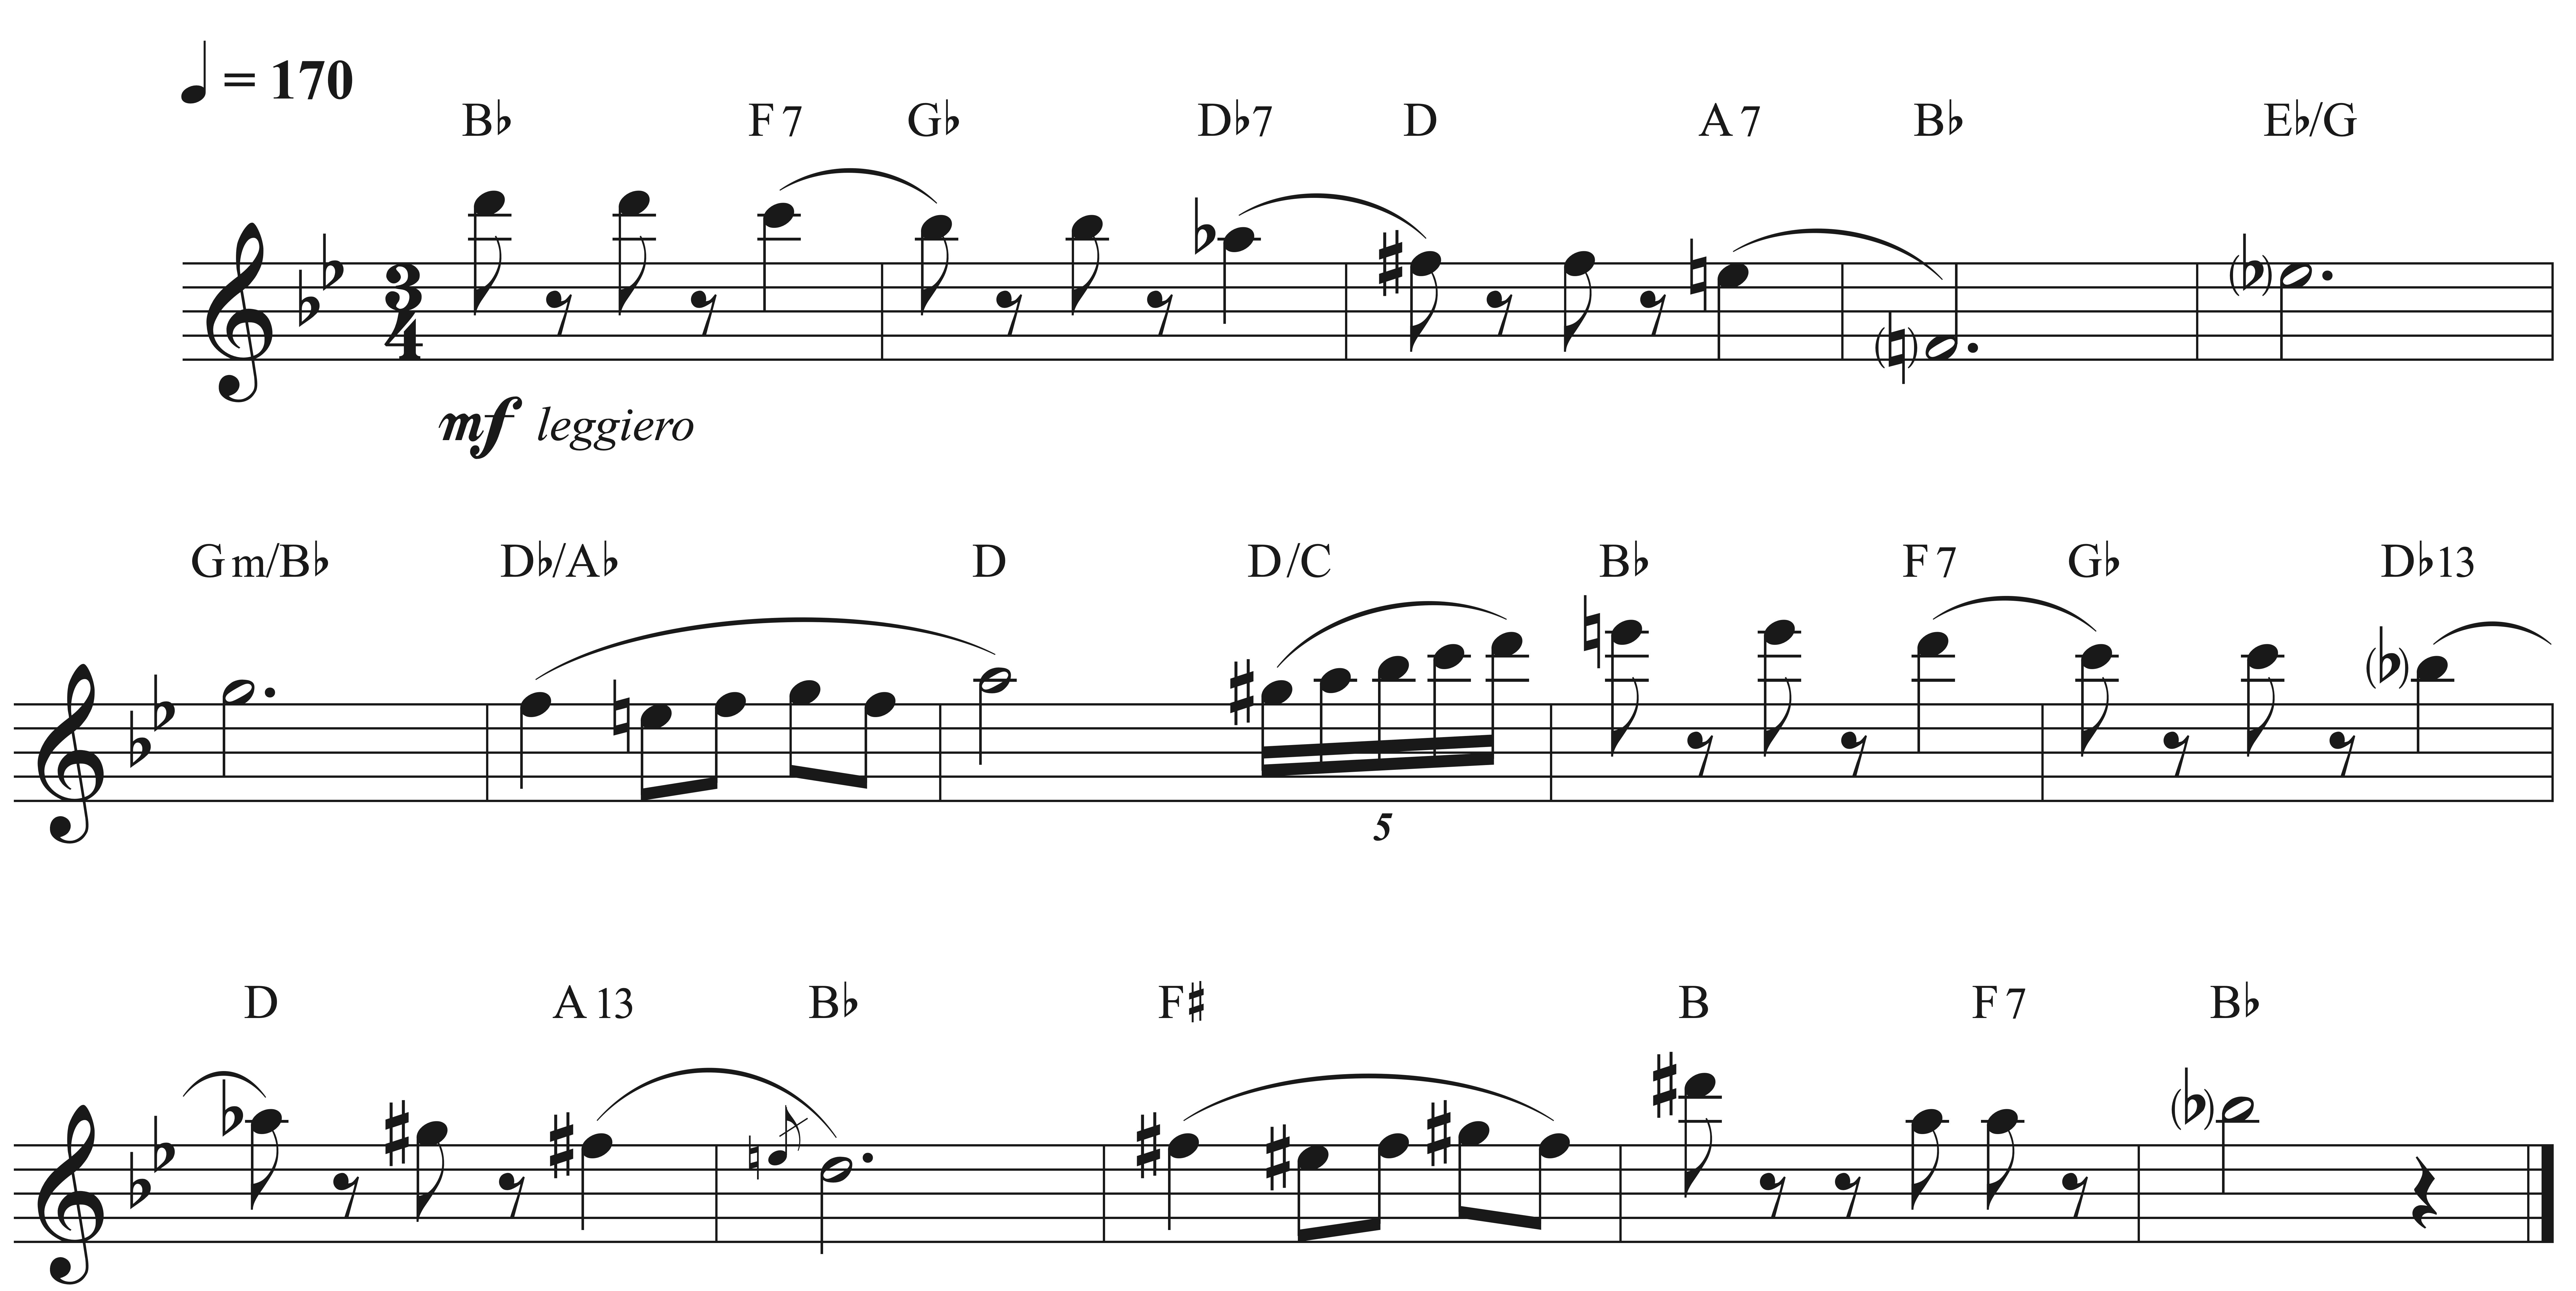
\includegraphics[width=\textwidth]{figures/images/Mahler 9 Giant Steps score.png}
        }
    \caption[Mahler's 9th Symphony, 2nd movement]{\small{A small excerpt from Mahler's 9th Symphony, 2nd movement: The melodic and harmonic contour propels through non-diatonic major thirds.}}
    \label{fig:mahler}
\end{figure}

\begin{figure}[ht]
    \centering
    \scalebox{0.9}{
    \includegraphics[width=\textwidth]{figures/images/giant steps score.png}
        }
    \caption[Giant Steps]{\small{John Coltrane's Giant Steps head: A testament to harmonic exploration, featuring rapid chord changes in non-diatonic major thirds.}}
    \label{fig:giant_steps}
\end{figure}

\begin{figure}
    \centering
    \scalebox{0.9}{
    \includegraphics[width=\textwidth]{figures/images/train interlude score.png}
        }
    \caption[Last Train Home]{\small{Pat Metheny's Last Train Home interlude.}}
    \label{fig:last_train}
\end{figure}
